
% vim:set ff=unix expandtab ts=2 sw=2:
{\textbf{RSCAPE}\hfill\normalsize{F. Gans \& M.D. Mahecha}}
\alert{\textit{Context:}}
\begin{itemize}
	\item Temperature is a key control of biogeochemical processes (e.g. on CO$_2$, CH$_4$, or N$_2$O production rates in soils)g.
	\item On seasonal and longer timescales other ecological factors e.g. substrate availability play an important role.
	\item The interaction of processes on different timescales is complicating the estimation of the temperature sensitivity of biogeochemcial processes.
\end{itemize}
 
\alert{\textit{Methods provided:}}
\begin{itemize}
	\item RSCAPE implements the "scale dependent parameter estimation” (SCAPE) principle (Mahecha et al. 2010).
    \item The user can choose amongst a wide range of 1) spectral decomposition methods and 2) standard or custom temperature sensitivity models.
    \item Full consideration to time-lagged responses and methodologcical uncertainties.
\end{itemize}
\vspace{1cm}
\begin{columns}
\column{.8\textwidth}
	\begin{figure}[tb]
	\begin{center}
		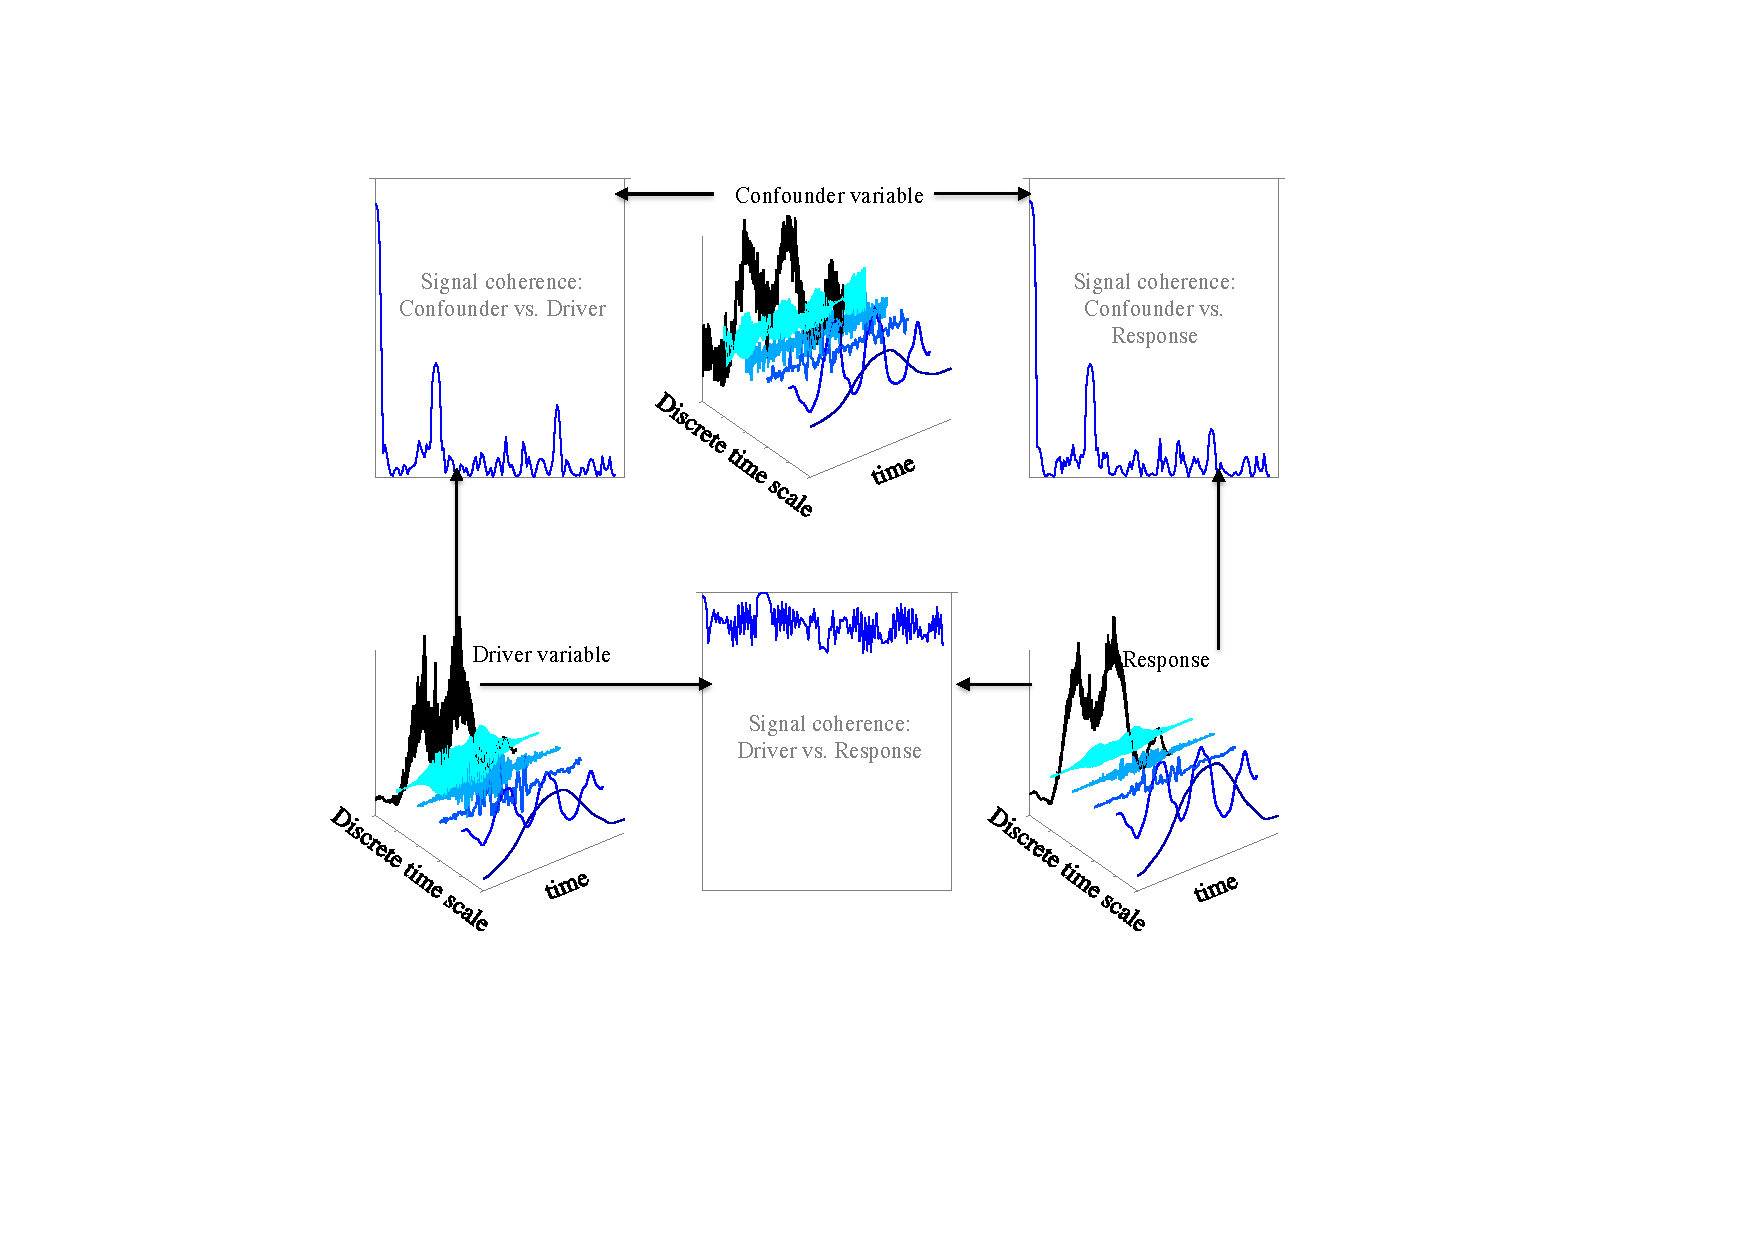
\includegraphics[width=.95\textwidth]{images/content/FIG1.pdf}
	\end{center}
	\end{figure}
\column{.2\textwidth}
\small{\textit{Conceptual problem solved by RSCAPE: The parameter estimtation problem (mapping from driver to response) is confounded on different time scales}}
\vspace{4cm}
	\begin{figure}[tb]
		
\includegraphics[width=.6\textwidth]{images/qrcode-RSCAPE.jpg}
	\end{figure}
\end{columns}
\vspace{1cm}
\hfill\large{\url{https://github.com/meggart/RSCAPE}}
\vfill
